\PassOptionsToPackage{unicode=true}{hyperref} % options for packages loaded elsewhere
\PassOptionsToPackage{hyphens}{url}
%
\documentclass[ignorenonframetext,]{beamer}
\usepackage{pgfpages}
\setbeamertemplate{caption}[numbered]
\setbeamertemplate{caption label separator}{: }
\setbeamercolor{caption name}{fg=normal text.fg}
\beamertemplatenavigationsymbolsempty
% Prevent slide breaks in the middle of a paragraph:
\widowpenalties 1 10000
\raggedbottom
\setbeamertemplate{part page}{
\centering
\begin{beamercolorbox}[sep=16pt,center]{part title}
  \usebeamerfont{part title}\insertpart\par
\end{beamercolorbox}
}
\setbeamertemplate{section page}{
\centering
\begin{beamercolorbox}[sep=12pt,center]{part title}
  \usebeamerfont{section title}\insertsection\par
\end{beamercolorbox}
}
\setbeamertemplate{subsection page}{
\centering
\begin{beamercolorbox}[sep=8pt,center]{part title}
  \usebeamerfont{subsection title}\insertsubsection\par
\end{beamercolorbox}
}
\AtBeginPart{
  \frame{\partpage}
}
\AtBeginSection{
  \ifbibliography
  \else
    \frame{\sectionpage}
  \fi
}
\AtBeginSubsection{
  \frame{\subsectionpage}
}
\usepackage{lmodern}
\usepackage{amssymb,amsmath}
\usepackage{ifxetex,ifluatex}
\usepackage{fixltx2e} % provides \textsubscript
\ifnum 0\ifxetex 1\fi\ifluatex 1\fi=0 % if pdftex
  \usepackage[T1]{fontenc}
  \usepackage[utf8]{inputenc}
  \usepackage{textcomp} % provides euro and other symbols
\else % if luatex or xelatex
  \usepackage{unicode-math}
  \defaultfontfeatures{Ligatures=TeX,Scale=MatchLowercase}
\fi
% use upquote if available, for straight quotes in verbatim environments
\IfFileExists{upquote.sty}{\usepackage{upquote}}{}
% use microtype if available
\IfFileExists{microtype.sty}{%
\usepackage[]{microtype}
\UseMicrotypeSet[protrusion]{basicmath} % disable protrusion for tt fonts
}{}
\IfFileExists{parskip.sty}{%
\usepackage{parskip}
}{% else
\setlength{\parindent}{0pt}
\setlength{\parskip}{6pt plus 2pt minus 1pt}
}
\usepackage{hyperref}
\hypersetup{
            pdftitle={CS5014 Machine Learning},
            pdfauthor={Lei Fang},
            pdfborder={0 0 0},
            breaklinks=true}
\urlstyle{same}  % don't use monospace font for urls
\newif\ifbibliography
\usepackage{longtable,booktabs}
\usepackage{caption}
% These lines are needed to make table captions work with longtable:
\makeatletter
\def\fnum@table{\tablename~\thetable}
\makeatother
\setlength{\emergencystretch}{3em}  % prevent overfull lines
\providecommand{\tightlist}{%
  \setlength{\itemsep}{0pt}\setlength{\parskip}{0pt}}
\setcounter{secnumdepth}{0}

% set default figure placement to htbp
\makeatletter
\def\fps@figure{htbp}
\makeatother

%\usepackage[latin1]{inputenc}

\usepackage{graphicx}
\usepackage{rotating}
%\setbeamertemplate{caption}[numbered]
\usepackage{hyperref}
\usepackage{caption}
\usepackage[normalem]{ulem}
%\mode<presentation>
\usepackage{wasysym}
\usepackage{amsmath}
\usepackage{mathtools}
\usepackage[skins,theorems]{tcolorbox}
\tcbset{highlight math style={enhanced,
  colframe=red,colback=white,arc=0pt,boxrule=1pt}}

\newcommand{\normal}[2]{\ensuremath{\mathcal{N}\left (#1,#2 \right )}}
\newcommand{\Gaussian}[3]{\ensuremath{\frac{1}{\sqrt{2\pi}#3}
\text{exp}\left \{-\frac{1}{2#3^2} (#1-#2)^2 \right \}}}
\newcommand{\argmax}{\operatornamewithlimits{argmax}}
\newcommand{\expo}[1]{\ensuremath{\text{exp}\left \{ #1 \right \}}}
\newcommand{\studentt}[4]{\ensuremath{\mathcal{T}_{#4}(#1,#2,#3)}}
\newcommand{\vv}[1]{\boldsymbol{#1}}
\newcommand{\Prb}{\ensuremath{\mathbb{P}}}
\newcommand{\studenttk}[4]{\ensuremath{\mathcal{T}_{#4}(#1,#2,#3)}}
\newcommand{\argmin}{\operatornamewithlimits{argmin}}
\newcommand{\NIG}{\mathcal{NIG}}
\newcommand{\N}{\mathcal{N}}
\newcommand{\T}{\mathcal{T}}
\newcommand{\IG}{\mathcal{IG}}
\newcommand{\IW}{\mathcal{IW}}
\newcommand{\NNIW}{\mathcal{NNIW}}
\newcommand{\vct}{\text{vec}}
\newcommand{\NN}{\mathcal{NN}}
\newcommand{\tr}{\text{tr}}
\newcommand{\di}[2]{\ensuremath{ #1^{(#2)}}}
\newcommand{\Di}[2]{\ensuremath{ \vv{#1}^{(#2)}}}

\newcommand{\E}[1]{\ensuremath{\mathbb{E}[#1]}}
\newcommand{\Var}[1]{\mathrm{Var}[#1]}
\newcommand{\Cov}[2]{\mathrm{Cov}[#1,#2]}
\newcommand{\Cor}[2]{\mathrm{Cor}[#1,#2]}


% \setbeamertemplate{navigation symbols}{}



%\titlegraphic{\includegraphics[width=0.3\paperwidth]{\string~/Dropbox/teaching/clemson-academic.png}}
\titlegraphic{\includegraphics[width=0.12\paperwidth]{crest.pdf}}
\setbeamertemplate{title page}[empty]

\setbeamerfont{subtitle}{size=\small}

\setbeamercovered{transparent}

\definecolor{clemsonpurple}{HTML}{522D80}
\definecolor{stablue}{HTML}{0052cc}
\definecolor{stared}{HTML}{ff4d4d}
\definecolor{clemsonorange}{HTML}{F66733}

\setbeamercolor{frametitle}{fg=stablue,bg=white}
\setbeamercolor{title}{fg=stablue,bg=white}
\setbeamercolor{local structure}{fg=stablue}
\setbeamercolor{section in toc}{fg=stablue,bg=white}
\setbeamercolor{subsection in toc}{fg=stared,bg=white}
\setbeamercolor{item projected}{fg=stablue,bg=white}
\setbeamertemplate{itemize item}{\color{stablue}$\bullet$}
\setbeamertemplate{itemize subitem}{\color{stablue}\scriptsize{$\bullet$}}
\let\Tiny=\tiny

%\makeatletter
%\setbeamertemplate{footline}{%
%\leavevmode
%\vbox{\begin{beamercolorbox}[dp=1.25ex,ht=2.75ex]{fg=black}%
%  \hspace*{1em}\insertsectionhead%
%  \ifx\insertsubsectionhead\@empty\relax\else$\quad\mid\quad$\insertsubsectionhead\fi :
%  \end{beamercolorbox}%
%  }%
%}
%\makeatother

\setbeamercolor{footercl}{fg=white,bg=stablue}
\setbeamerfont{stafont}{size = \large}
\setbeamerfont{footerfont}{size = \tiny}
% \makeatother
% \setbeamertemplate{footline}
% {
%   \leavevmode%
%   \hbox{%
%   \begin{beamercolorbox}[wd=.5\paperwidth,ht=5ex,dp=1ex, left]{footercl}%
%     \usebeamerfont*{stafont}\hspace*{1ex}\insertshortinstitute
%   \end{beamercolorbox}%
%   \begin{beamercolorbox}[wd=.25\paperwidth,ht=5ex,dp=1ex,center]{footercl}%
%     \usebeamerfont*{footerfont}\insertshorttitle\hspace*{1ex} \insertframenumber{}
%   \end{beamercolorbox}%
%   \begin{beamercolorbox}[wd=.25\paperwidth,ht=5ex,dp=1ex,right]{footercl}%
%    \includegraphics[height=5ex]{stalogo.png}
%   \end{beamercolorbox}}%
%   \vskip0pt%
% }
% \makeatletter
\makeatletter
\setbeamertemplate{footline}
{
  \leavevmode%
  \hbox{%
  \fontsize{13}{13}\fontfamily{ppl}\selectfont
  \begin{beamercolorbox}[wd=.5\paperwidth,ht=2.25ex,dp=1ex,left]{footercl}%
    \usebeamerfont{author in head/foot}\hspace*{1ex}\insertshortinstitute
   \end{beamercolorbox}%
   \begin{beamercolorbox}[wd=.25\paperwidth,ht=2.25ex,dp=1ex,right]{footercl}%
    % \hfill\hfill\hfill\hfill\hfill\hfill\hfill\hfill\hfill\hfill
    \parbox{.25\paperwidth}{\fontfamily{cmss}\selectfont{\hfill\hfill \usebeamerfont{footerfont}\insertshorttitle~\insertframenumber{}}}
  \end{beamercolorbox}%
  \begin{beamercolorbox}[wd=.25\paperwidth,ht=2.25ex,dp=1ex,left]{footercl}%
    \parbox{.25\paperwidth}{\hfill\includegraphics[height=1cm]{stalogo.png}}% original: 2ex
  \end{beamercolorbox}}%
  \vskip0pt%
}
\makeatother

\setbeamertemplate{navigation symbols}{}

% \AtBeginDocument{\author[L. Fang]{Lei Fang} \institute[www.st-andrews.ac.uk]{School of Computer Science, University of St Andrews}}

% \newcommand{\Ffootline}{%                   %%defines a new command called \Ffootline
% %\insertshortauthor,                         %%puts the abbreviated form of the author's name in the left corner
% \insertshorttitle,
% \insertshortinstitute, 
% \insertshortdate %%puts the abbreviated form of the author's institution in the middle
% \hfill
% \insertsection,
% \insertframenumber/\inserttotalframenumber} %%includes the current slide number over the total slide number in the right corner
% \setbeamertemplate{footline}{%              %%sets the options for the footline
% \usebeamerfont{structure}                   %%uses the same fonts adopted for the structure of the presentation 
% \Tiny\hspace*{4mm} \Ffootline \hspace{4mm}  %%sets the size of the font to Tiny and includes the content of the \Ffootline
% }                                           %%command leaving a margin of 4mm to the right and left of the content.



\AtBeginPart{}
\AtBeginSection{}
\AtBeginSubsection{}
\AtBeginSubsubsection{}
\setlength{\emergencystretch}{0em}
\setlength{\parskip}{0pt}
\AtBeginDocument{\author[L. Fang]{Lei Fang} \title[L3 Linear Regression]{CS5014 Machine Learning}\institute[www.st-andrews.ac.uk]{School of Computer Science, University of St Andrews}}

\title{CS5014 Machine Learning}
\providecommand{\subtitle}[1]{}
\subtitle{Lecture 3 Linear Regression}
\author{Lei Fang}
\date{Spring 2021}

\begin{document}
\frame{\titlepage}

\hypertarget{introduction}{%
\section{Introduction}\label{introduction}}

\begin{frame}{Topics for today}
\protect\hypertarget{topics-for-today}{}

Linear regression

\begin{itemize}
\tightlist
\item
  matrix notation
\item
  normal equation and closed form solution

  \begin{itemize}
  \tightlist
  \item
    vector calculus perspective
  \item
    linear algebra perspective: projection
  \end{itemize}
\item
  gradient descent

  \begin{itemize}
  \tightlist
  \item
    a more general solution
  \end{itemize}
\end{itemize}

\end{frame}

\begin{frame}{Supervised learning vs unsupervised learning}
\protect\hypertarget{supervised-learning-vs-unsupervised-learning}{}

Supervised learning

\begin{itemize}
\tightlist
\item
  dataset contains both predictors \(\vv{x} = \{x_1, \ldots, x_n\}\) and
  targets \({y}\)
\item
  regression: \(y\) is continuous

  \begin{itemize}
  \tightlist
  \item
    e.g.~predict your height based your weight: \(n=1\), and \(x_1\) is
    height, \(y\) is weight
  \end{itemize}
\item
  classification: \(y\) is categorical

  \begin{itemize}
  \tightlist
  \item
    e.g.~predict adult or child \(y=\{A, C\}\) based on height
    measurement \(\vv{x}\)
  \end{itemize}
\end{itemize}

\bigskip

Unsupervised learning

\begin{itemize}
\tightlist
\item
  dataset formed only with predictors \(\vv{x}\): no targets
\item
  aim: understand the underlying structure of \(\vv{x}\)
\item
  typical learning: clustering, dimension reduction etc.
\end{itemize}

\end{frame}

\begin{frame}{Regression: Catheter dataset}
\protect\hypertarget{regression-catheter-dataset}{}

Task: predict a patient's catheter \emph{length} (target) by predictors:
\emph{height} and \emph{weight} \vspace{-0.2cm} \footnotesize

\begin{longtable}[]{@{}rrr@{}}
\toprule
height.in & weight.lbs & length.cm\tabularnewline
\midrule
\endhead
42.8 & 40.0 & 37\tabularnewline
63.5 & 93.5 & 50\tabularnewline
37.5 & 35.5 & 34\tabularnewline
39.5 & 30.0 & 36\tabularnewline
45.5 & 52.0 & 43\tabularnewline
38.5 & 17.0 & 28\tabularnewline
43.0 & 38.5 & 37\tabularnewline
22.5 & 8.5 & 20\tabularnewline
37.0 & 33.0 & 34\tabularnewline
23.5 & 9.5 & 30\tabularnewline
33.0 & 21.0 & 38\tabularnewline
58.0 & 79.0 & 47\tabularnewline
\bottomrule
\end{longtable}

\end{frame}

\begin{frame}{Regression: Catheter dataset}
\protect\hypertarget{regression-catheter-dataset-1}{}

The regression problem can be formed as:
\[y^{(i)} =f(\vv{x}^{(i)}; \vv{\theta}) + e^{(i)}\]

\begin{itemize}
\tightlist
\item
  \(f\) is a model that predict \(y^{(i)}\) from \(\vv{x}^{(i)}\)

  \begin{itemize}
  \tightlist
  \item
    \(i = 1,\ldots,m\): index of data samples (row index),
  \item
    \(m\) is the total training size
  \end{itemize}
\item
  \(\vv{x}^{(i)} = [x_{1}^{(i)}, \ldots, x^{(i)}_n]^T\) is a
  \(n\times 1\) vector:

  \begin{itemize}
  \tightlist
  \item
    \(n\): number of predictors (columns)
  \end{itemize}
\item
  e.g. \(y^{(1)} = 37\) and \(\vv{x}^{(1)} = [42.8, 40]^T\)
\item
  \(\vv{\theta}\) is the model parameter
\item
  \(e^{(i)}\) is the prediction difference of the \(i\)-th entry
\end{itemize}

\end{frame}

\begin{frame}{Linear regression}
\protect\hypertarget{linear-regression}{}

If we further assume the relationship is linear, i.e. \begin{align*}
f(\vv{x}^{(i)}; \vv{\theta}) &= \theta_0 + \theta_1  x^{(i)}_{1} + \ldots +\theta_{n} x^{(i)}_n \\
&= [\theta_0, \theta_1, \ldots, \theta_n] \begin{bmatrix}1\\ x^{(i)}_1\\ \vdots\\ x^{(i)}_n\end{bmatrix} = \vv{\theta}^T\vv{x}^{(i)}
\end{align*} the regression is called \textbf{linear regression}

\bigskip

\begin{itemize}
\tightlist
\item
  a dummy predictor \(x_0^{(1)}=1\) is added to \(\vv{x}^{(i)}\)
\end{itemize}

\end{frame}

\begin{frame}{Linear regression: least squared error}
\protect\hypertarget{linear-regression-least-squared-error}{}

The prediction error is

\[e^{(i)} = y^{(i)} - f(\vv{x}^{(i)}; \vv{\theta}) = y^{(i)} - \vv{\theta}^T\vv{x}^{(i)}\]

The sum of squared errors is

\[L(\vv{\theta}) = \sum_{i=1}^m (y^{(i)} - \vv{\theta}^T\vv{x}^{(i)})^2\]

Learning objective is then to minimise the cost function

\[\hat{\theta} = \argmin_{\vv{\theta}} L(\vv{\theta}; \{\vv{x}^{(i)}, y^{(i)}\}_1^m)\]

\end{frame}

\begin{frame}{Linear models and hyperplane}
\protect\hypertarget{linear-models-and-hyperplane}{}

Geometrically, linear function

\[f(\vv{x}; \vv{\theta}) = \theta_0 + \theta_1  x_{1} + \ldots +\theta_{n} x_n = \vv{\theta}^T\vv{x}\]
is a hyperplane

\begin{itemize}
\tightlist
\item
  \(\vv{\theta}\) is the gradient vector \(\nabla_{\vv{x}} f\): the
  greatest ascent direction of \(f\)
\item
  minising \(L\) means to find a hyperplane that \emph{fits} the data
  best \bigskip
\end{itemize}

\begin{center}\includegraphics[width=1\linewidth]{lecture3_files/figure-beamer/unnamed-chunk-4-1} \end{center}

\end{frame}

\begin{frame}{How to optimise \(L(\vv{\theta})\) ?}
\protect\hypertarget{how-to-optimise-lvvtheta}{}

Vector calculus is our friend:

\begin{itemize}
\tightlist
\item
  find the gradient \(\nabla_{\vv{\theta}} L\)
\item
  set it to zero
\end{itemize}

\bigskip

In matrix notation, let
\[\vv{y} = \begin{bmatrix} y^{(1)}\\ y^{(2)}\\ \vdots\\ y^{(m)} \end{bmatrix},  \vv{X} = \begin{bmatrix}
1 & x_1^{(1)} & \ldots & x_{n}^{(1)}\\
1 & x_1^{(2)} & \ldots & x_{n}^{(2)} \\
\vdots & \vdots & & \vdots \\
1 & x_1^{(m)} & \ldots & x_{n}^{(m)}
\end{bmatrix} = \begin{bmatrix} \text{---} (\vv{x}^{(1)})^T \text{---} \\
\text{---} (\vv{x}^{(2)})^T \text{---} \\
\vdots \\
 \text{---} (\vv{x}^{(m)})^T \text{---}
\end{bmatrix}, \vv{\theta} =\begin{bmatrix} \theta_0\\ \theta_1\\ \vdots \\ \theta_n\end{bmatrix}\]
then

\[\vv{e} = \begin{bmatrix} e^{(1)} \\ \vdots \\ e^{(m)}\end{bmatrix} = \begin{bmatrix} y^{(1)}\\ \vdots\\ y^{(m)} \end{bmatrix} - \begin{bmatrix} (\vv{x}^{(1)})^T \vv{\theta} \\
\vdots \\
 (\vv{x}^{(m)})^T \vv{\theta}
\end{bmatrix} = \vv{y} - \vv{X\theta}\]

\end{frame}

\begin{frame}{Find the gradient: \(\nabla_{\vv{\theta}}L\)}
\protect\hypertarget{find-the-gradient-nabla_vvthetal}{}

\[L(\vv{\theta}) = \sum_{i=1}^m (y^{(i)} - \vv{\theta}^T\vv{x}^{(i)})^2 = (\vv{y} -\vv{X\theta})^T(\vv{y}-\vv{X\theta}) = \vv{e}^T\vv{e}\]

\begin{itemize}
\tightlist
\item
  it is a quadratic form (a quadratic form is
  \(\vv{x}^T \vv{A} \vv{x}\): a row vector times a matrix times a column
  vector, the result is a scalar !)
  \[\frac{\partial L}{\partial \vv{e}} \equiv \nabla_{\vv{e}} L = \nabla_{\vv{e}} (\vv{e}^T\vv{I}\vv{e}) = 2(\vv{Ie})^T = 2\vv{e}^{T}\]
\item
  but we need \(\nabla_{\vv{\theta}}L\), to apply chain rule we need:
  \[\frac{\partial \vv{e}}{\partial \vv{\theta}} = \frac{\partial (\vv{y}- \vv{X\theta})}{\partial \vv{\theta}} =-\vv{X}\]
\item
  finally,
  \[\nabla_{\vv{\theta}} L = \frac{\partial L}{\partial \vv{e}}\frac{\partial \vv{e}}{\partial \vv{\theta}} = 2\vv{e}^{T}(-\vv{X}) = -2(\vv{y}-\vv{X\theta})^{T}\vv{X} \]
\end{itemize}

\end{frame}

\begin{frame}{A few notes on vector derivatives: gradient as row vector}
\protect\hypertarget{a-few-notes-on-vector-derivatives-gradient-as-row-vector}{}

For vector to scalar function \(f(\vv{\beta}): R^m \rightarrow R\): the
gradient

\[\nabla_{\vv{x}}f = \left [\frac{\partial f}{\partial \beta_1}, \ldots, \frac{\partial f}{\partial \beta_m}\right ]\in R^{1\times m}\]

\begin{itemize}
\tightlist
\item
  we adopt the convention: gradients as \emph{row vectors}
\item
  e.g.~for \(L(\vv{e}) = \vv{e}^T\vv{e}\):
  \(\nabla_{\vv{e}} L = 2\vv{e}^{T}\)

  \begin{itemize}
  \tightlist
  \item
    \(\vv{e}\) is defined as a column vector, its transpose is a row
    vector
  \end{itemize}
\end{itemize}

\end{frame}

\begin{frame}{A few notes on vector derivatives: vector valued
functions}
\protect\hypertarget{a-few-notes-on-vector-derivatives-vector-valued-functions}{}

The convention generalises well to
\(\vv{g}(\vv{\theta}): R^n\rightarrow R^m\) functions: e.g.

\[\vv{e} = \vv{g}(\vv{\theta}) =\vv{y} - \vv{X}\vv{\theta}\]

\begin{itemize}
\tightlist
\item
  a vector to vector function: \(R^n\rightarrow R^m\)
\item
  each
  \(e^{(i)} = y^{(i)}- (\vv{x}^{(i)})^T \vv{\theta} = y^{(i)}- \sum_{j=1}^n ({x}^{(i)}_j) {\theta_j}\)
  is \(R^n \rightarrow R\)

  \begin{itemize}
  \tightlist
  \item
    its gradient is a row vector (\(\theta_0\) and \(x_0\) are dropped
    here for convenience)
    \[\nabla_{\vv{\theta}} e^{(i)} = \left [\frac{\partial e^{(i)}}{\partial\theta_1}, \ldots, \frac{\partial e^{(i)}}{\partial\theta_n}\right ] = \left [-x_1^{(i)}, \ldots, -x_n^{(i)} \right]\]
  \end{itemize}
\item
  the gradient for \(\nabla_{\vv{\theta}} \vv{g}(\vv{\theta})\) is
  \[\nabla_{\vv{\theta}} \vv{g}(\vv{\theta})  = \begin{bmatrix} \nabla_{\vv{\theta}} e^{(1)} \\ \vdots \\ \nabla_{\vv{\theta}} e^{(m)} \end{bmatrix}  = \begin{bmatrix} -x_1^{(1)}, \ldots, -x_n^{(1)}  \\ \vdots \\ -x^{(m)}_1, \ldots, -x^{(m)}_n  \end{bmatrix}= -\vv{X}\]
\end{itemize}

\end{frame}

\begin{frame}{}
\protect\hypertarget{section}{}

\begin{itemize}
\tightlist
\item
  easier to use chain rule (matrix shapes need to match to multiple!):
  \[\nabla_{\vv{\theta}} L = \frac{\partial L}{\partial \vv{e}}\frac{\partial \vv{e}}{\partial \vv{\theta}} = 2\vv{e}^{T}(-\vv{X}) = -2(\vv{y}-\vv{X\theta})^{T}\vv{X} \]
  is still a row vector
\end{itemize}

\end{frame}

\begin{frame}{Some useful gradients}
\protect\hypertarget{some-useful-gradients}{}

\[\frac{\partial (\vv{b} + \vv{Ax})}{\partial \vv{x}} = \vv{A};\;\; \frac{\partial (\vv{b} - \vv{Ax})}{\partial \vv{x}} = -\vv{A}\]

\begin{equation*}
\frac{\partial \vv{x}^T \vv{a}}{\partial \vv{x}}= \frac{\partial \vv{a}^T \vv{x}}{\partial \vv{x}} = \vv{a}^T  
\end{equation*}

\[\frac{\partial\vv{x}^T\vv{B}\vv{x}}{\partial\vv{x}} = \vv{x}^{T}(\vv{B}+ \vv{B}^{T});\;\; \frac{\partial\vv{x}^T\vv{W}\vv{x}}{\partial\vv{x}} = 2\vv{x}^{T}\vv{W}; \; \vv{W}\text{ is symmetric}\]
\[\frac{\partial\vv{x}^T\vv{x}}{\partial\vv{x}} = 2\vv{x}^{T}\]
\[\frac{\partial(\vv{x}-\vv{As})^T\vv{W}(\vv{x}-\vv{As})}{\partial\vv{s}} = -2(\vv{x}-\vv{As})^T\vv{WA},\; \vv{W} \text{ is symmetric}\]

\[\frac{\partial a^T\vv{X}\vv{b}}{\partial\vv{X}} = \vv{ab}^{T}\]

\end{frame}

\begin{frame}{Normal equation for linear regression}
\protect\hypertarget{normal-equation-for-linear-regression}{}

To find the minimum, set \(\nabla_{\vv{\theta}} L =\vv{0}\), we have the
\textbf{Normal Equations}:

\begin{align*}
2(\vv{y}-\vv{X\theta})^{T}\vv{X} = \vv{0}^T &\Rightarrow 2\vv{X}^T (\vv{y}-\vv{X\theta})= \vv{0} \\ &\Rightarrow \vv{X}^T\vv{X}\vv{\theta} = \vv{X}^T\vv{y}
\end{align*} \bigskip

Assuming \(\vv{X}^T\vv{X}\) is invertible (nonsingular), we have the
closed-form solution

\[\vv{\theta}_{ls} = (\vv{X}^T\vv{X})^{-1}\vv{X}^{T}\vv{y}\]

\begin{itemize}
\tightlist
\item
  ``ls'' means least square
\end{itemize}

\end{frame}

\begin{frame}{\((\vv{X}^T\vv{X})\) singular case}
\protect\hypertarget{vvxtvvx-singular-case}{}

\(\vv{X}^T\vv{X}\) has to be invertible or nonsingular

\begin{itemize}
\tightlist
\item
  otherwise, the matrix is called ill-conditioned
\item
  like dividing a number by \(0\)
\end{itemize}

\bigskip

Note that \(\text{rank}(\vv{X^TX}) = \text{rank}(\vv{X})\)

\begin{itemize}
\tightlist
\item
  so \(\vv{X}\) has linearly dependent columns \(\Rightarrow\)
  \(\vv{X}^T\vv{X}\) singular
\item
  e.g.~the same feature but measured in different units, like inch or
  cm: \(\vv{x}_h =k\times \vv{x}_i\)
\item
  also called highly correlated features (redundant feature for
  regressing \(\vv{y}\))
\item
  or more general, one of the feature is a linear combination of the
  rest
\end{itemize}

\bigskip

Deal with nonsingular \(\vv{X}^T\vv{X}\)

\begin{itemize}
\tightlist
\item
  remove problematic features
\item
  dimension reduction first
\item
  regularization (more on this later)
\end{itemize}

\end{frame}

\begin{frame}{Normal equation: projection view of \(\text{col}(X)\)}
\protect\hypertarget{normal-equation-projection-view-of-textcolx}{}

Derivative is way too complicated! Let's see something cooler :-)
\begin{align*}\footnotesize \vv{X\theta} = \begin{bmatrix}
1 & x_1^{(1)} & \ldots & x_{n}^{(1)}\\
1 & x_1^{(2)} & \ldots & x_{n}^{(2)} \\
\vdots & \vdots & & \vdots \\
1 & x_1^{(m)} & \ldots & x_{n}^{(m)}
\end{bmatrix} \begin{bmatrix} \theta_0\\ \theta_1\\ \vdots \\ \theta_n\end{bmatrix} = \theta_0 \begin{bmatrix}1 \\ 1\\ \vdots \\ 1\end{bmatrix}+ \theta_1 \begin{bmatrix}x^{(1)}_1 \\ x^{(2)}_1\\ \vdots\\ x^{(m)}_1\end{bmatrix} +\ldots+  \theta_n \begin{bmatrix}x^{(1)}_n \\ x^{(2)}_n\\ \vdots\\ x^{(m)}_n\end{bmatrix} \end{align*}
\[=\theta_0 \vv{x}_0 + \theta_{1} \vv{x}_1 +\ldots + \theta_n \vv{x}_n\]

\begin{itemize}
\tightlist
\item
  linear combination of column vectors of \(\vv{X}\)
\end{itemize}

\bigskip

what does \(\vv{y} = \vv{X\theta}\) solve ?

\begin{itemize}
\tightlist
\item
  whether \(\vv{y}\) can be represented as a linear combination of
  column vectors of \(\vv{X}\)
\item
  or \(\vv{y}\) lives in the column space or not:
  \(\vv{y} \in? \text{span}(\{\vv{x}_0, \vv{x}_1, \ldots, \vv{x}_n\})\)
\end{itemize}

\end{frame}

\begin{frame}{}
\protect\hypertarget{section-1}{}

\(\vv{y}= \vv{X\theta}\) is over determined: \(m>n\)

\begin{itemize}
\tightlist
\item
  usually
  \(\vv{y} \notin \text{span}(\{\vv{x}_0, \vv{x}_1, \ldots, \vv{x}_n\})\)
\item
  but we can find its best approximation in that span:
  \[\hat{\vv{y}} = \vv{X}\vv{\theta} \in \text{span}(\{\vv{x}_0, \vv{x}_1, \ldots, \vv{x}_n\})\]
\item
  and minimise \(\vv{e} = \vv{y}-\hat{\vv{y}}\)
\end{itemize}

\begin{figure}
    \centering
    \includegraphics[width = 0.8\textwidth]{./projview1.png}
 % \caption{Awesome figure}
\end{figure}

\end{frame}

\begin{frame}{}
\protect\hypertarget{section-2}{}

\vspace{-0.3cm}
\begin{figure}
    \centering
   \includegraphics[width = 0.47\textwidth, trim=1.2cm 0.5cm 0.8cm 0cm, clip]{./projview1.png}  \includegraphics[width = 0.51\textwidth, trim=0.5cm 0.5cm 0.5cm 0cm, clip]{./projview2.png}
 % \caption{Awesome figure}
\end{figure}

\(\vv{e}\) is minimised when \(\hat{\vv{y}}\) is \(\vv{y}\)'s projection
in \(\vv{span}(\{\vv{x}\})\), or
\[\vv{e} \perp \text{span}(\{\vv{x}_0, \vv{x}_1, \ldots, \vv{x}_n\}) \text{ or}\]
\[\begin{cases} \vv{x}_0 ^T \vv{e} = 0 \\ \vv{x}_1 ^T \vv{e} = 0 \\ \ldots\\ \vv{x}_n ^T \vv{e} =0  \end{cases}\Rightarrow \vv{X}^T\vv{e} =\vv{0} \Rightarrow  \vv{X}^T(\vv{y}-\vv{X\theta}) =\vv{0}\]

\end{frame}

\begin{frame}{Hat matrix}
\protect\hypertarget{hat-matrix}{}

The projected vector :
\[\hat{\vv{y}} = \vv{X}\vv{\theta} = \underbrace{\vv{X} (\vv{X}^{T}\vv{X})^{-1}\vv{X}^{T}}_{\text{hat matrix}}\vv{y}\]

\begin{itemize}
\tightlist
\item
  ``it gives \(\vv{y}\) a hat'': so given this name
\item
  it is also a projection matrix: it projects \(\vv{y}\) to its
  projection \(\hat{\vv{y}}\)
\item
  note that for all projection matrix \(\vv{P}\), \(\vv{PP} =\vv{P}\):
\end{itemize}

\[(\vv{X} (\vv{X}^{T}\vv{X})^{-1}\vv{X}^{T})(\vv{X} (\vv{X}^{T}\vv{X})^{-1}\vv{X}^{T}) =\vv{X} (\vv{X}^{T}\vv{X})^{-1}\vv{X}^{T}\]

\begin{itemize}
\tightlist
\item
  \(\vv{PP}\ldots\vv{P} =\vv{P}\)
\item
  \(\vv{PP}\ldots\vv{Px} = \vv{Px}\) as expected: further projections
  have no effect
\end{itemize}

\end{frame}

\begin{frame}{Gradient descent}
\protect\hypertarget{gradient-descent}{}

For most models, \(\nabla_{\vv{\theta}} L(\vv{\theta}) = \vv{0}\) has no
closed form solution

\begin{itemize}
\tightlist
\item
  linear regression is probably the only exception
\end{itemize}

\bigskip

Gradient descent provides a more general algorithm

\bigskip

Remember what gradient \(\nabla_{\vv{\theta}} L(\vv{\theta}_t)\) is ?

\begin{itemize}
\tightlist
\item
  it points to the greatest ascent direction of \(L\) at location
  \(\vv{\theta}_t\)
\item
  gradient descent algorithm is simple
\item
  at each \(t\), we move by the steepest descent direction
\item
  looping until converge:
\end{itemize}

\[\vv{\theta}_{t+1} \leftarrow  \vv{\theta}_{t} - \alpha \nabla_{\vv{\theta}}L(\vv{\theta}_t)\]

\end{frame}

\begin{frame}{Gradient recap}
\protect\hypertarget{gradient-recap}{}

For function \(L(\vv{\theta})\)

\begin{itemize}
\tightlist
\item
  the gradient \(\nabla_{\vv{\theta}}L(\vv{\theta})\) points to the
  ascent direction

  \begin{itemize}
  \tightlist
  \item
    vector field: input a location, output a direction
  \end{itemize}
\item
  the opposite \(-\nabla_{\vv{\theta}}L(\vv{\theta})\) points to the
  steepest descent direction
\item
  \(\vv{\theta}_{t} - \alpha \nabla_{\vv{\theta}}L(\vv{\theta}_t)\)
  moves to a new position in the input space
\end{itemize}

\begin{columns}
    \begin{column}{0.48\textwidth}

\begin{center}\includegraphics[width=1\linewidth]{lecture3_files/figure-beamer/unnamed-chunk-5-1} \end{center}
    \end{column}
    \begin{column}{0.48\textwidth}
      \begin{figure}
    \centering
    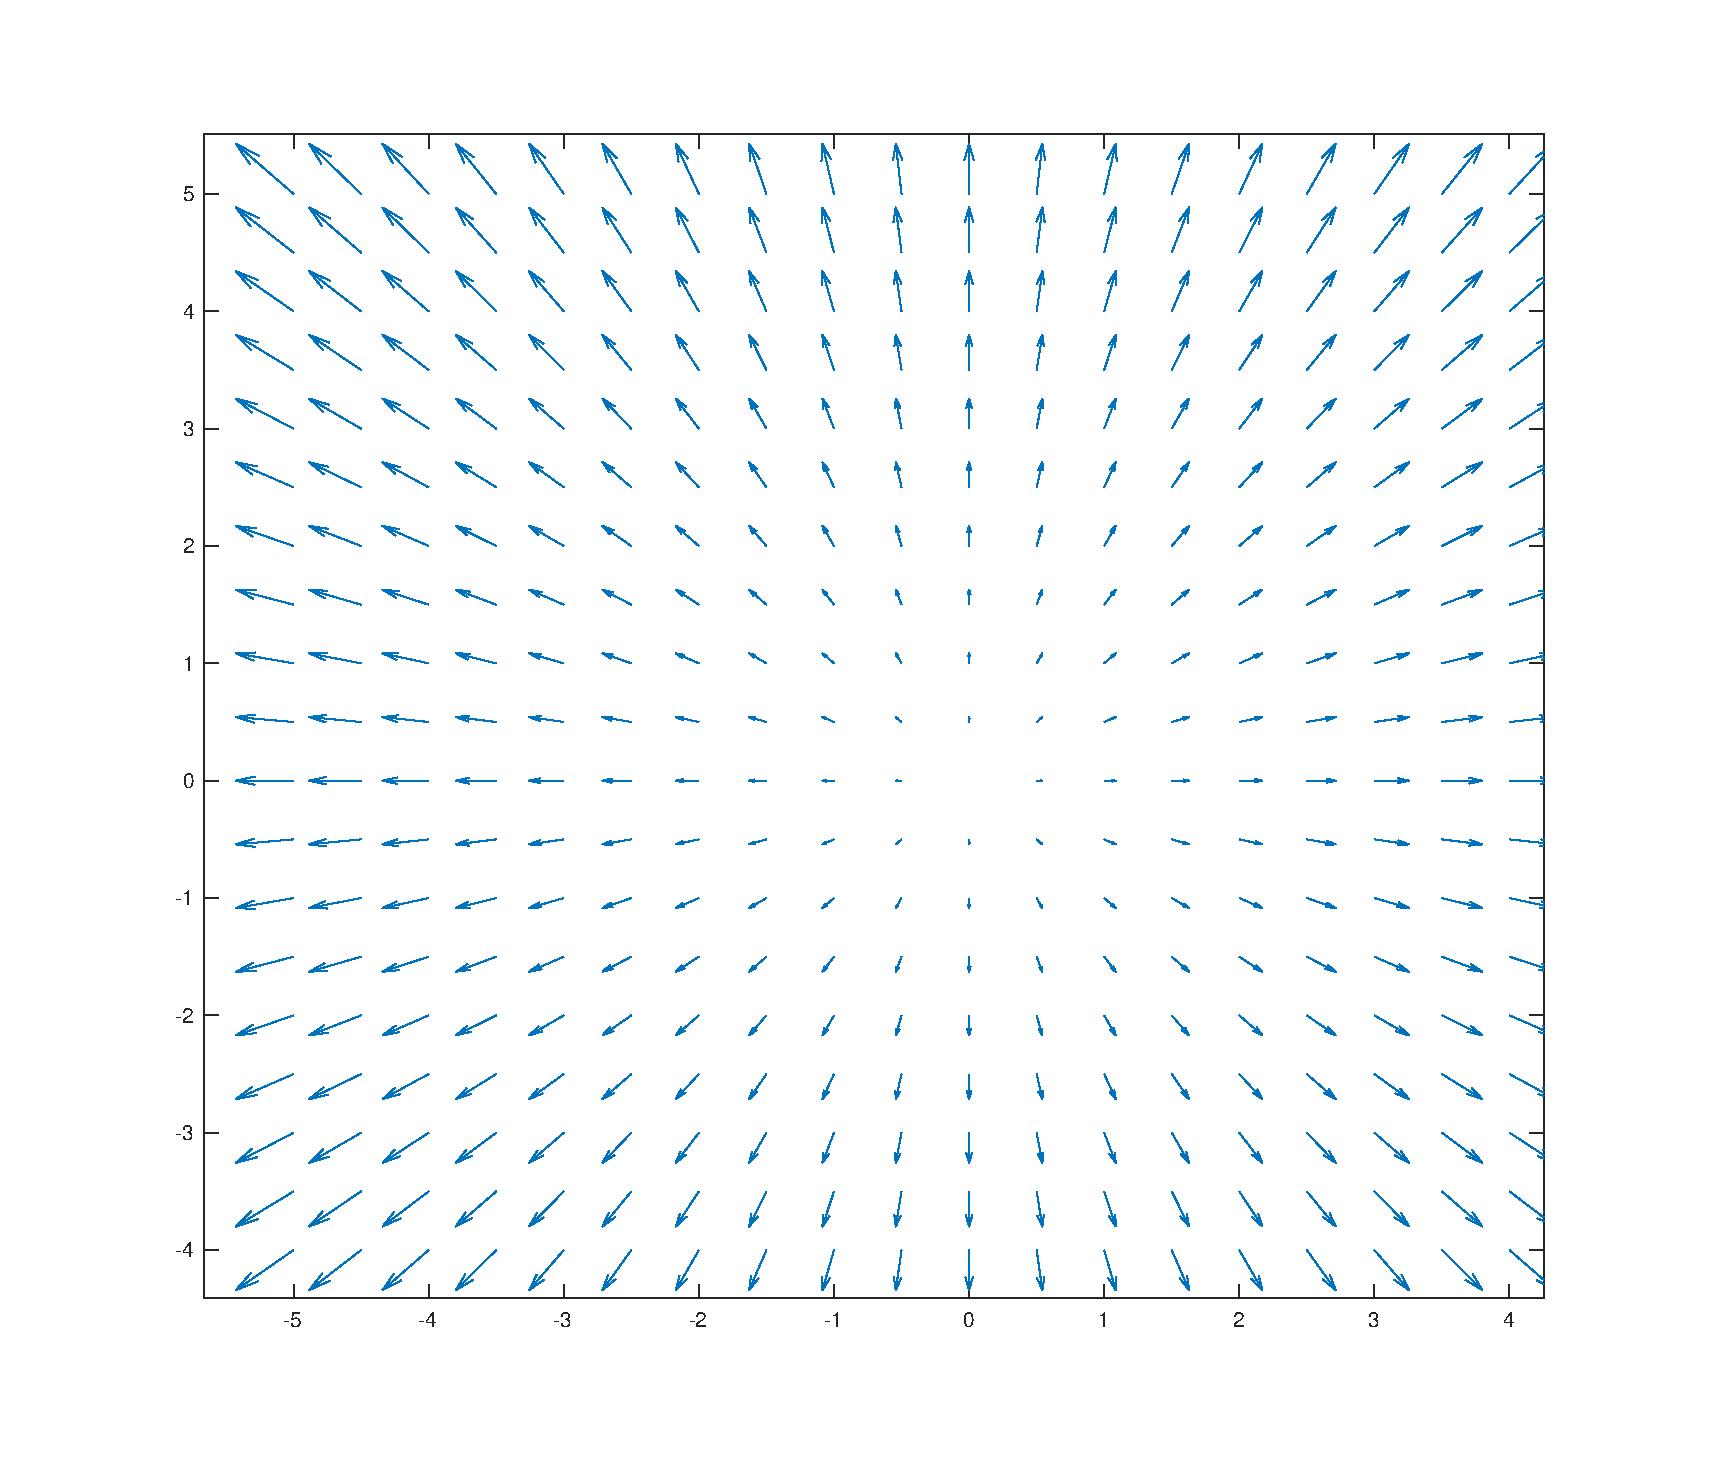
\includegraphics[width = \textwidth]{./gradvecfield.eps}
 % \caption{Awesome figure}
\end{figure}
    \end{column}
\end{columns}

\end{frame}

\begin{frame}{Gradient descent: step by step}
\protect\hypertarget{gradient-descent-step-by-step}{}

Initialisation: \(\vv{\theta}_0 = \vv{0}\);

\begin{itemize}
\tightlist
\item
  \(L = 1369.33\)
\end{itemize}

\begin{center}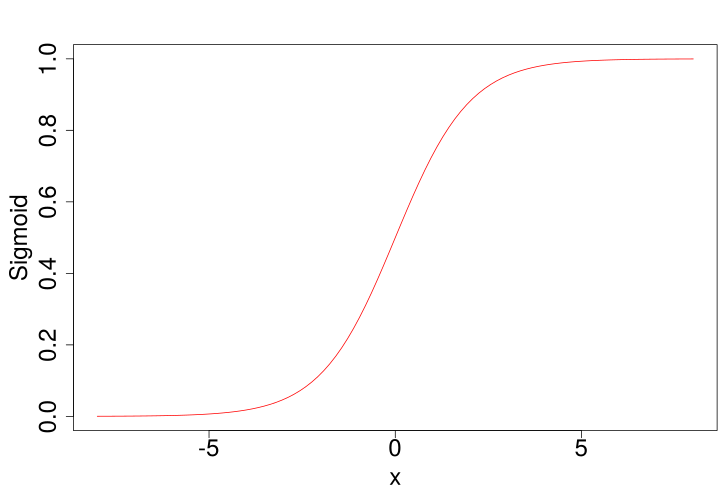
\includegraphics[width=0.5\linewidth]{lecture3_files/figure-beamer/unnamed-chunk-7-1} \end{center}

\end{frame}

\begin{frame}{Gradient descent: step by step}
\protect\hypertarget{gradient-descent-step-by-step-1}{}

Step 1: \(\vv{\theta}_1 = [0.007, 0.308, 0.311]\)

\begin{itemize}
\tightlist
\item
  \(L = 168\)
\end{itemize}

\begin{center}\includegraphics[width=0.5\linewidth]{lecture3_files/figure-beamer/unnamed-chunk-8-1} \end{center}

\end{frame}

\begin{frame}{Gradient descent: step by step}
\protect\hypertarget{gradient-descent-step-by-step-2}{}

Step 2: \(\vv{\theta}_2 = [0.010, 0.395, 0.381]\)

\begin{itemize}
\tightlist
\item
  \(L = 89.22\)
\end{itemize}

\begin{center}\includegraphics[width=0.5\linewidth]{lecture3_files/figure-beamer/unnamed-chunk-9-1} \end{center}

\end{frame}

\begin{frame}{Gradient descent: step by step}
\protect\hypertarget{gradient-descent-step-by-step-3}{}

Step 3: \(\vv{\theta}_3 = [0.011,0.425,0.391]\)

\begin{itemize}
\tightlist
\item
  \(L = 81.78\)
\end{itemize}

\begin{center}\includegraphics[width=0.5\linewidth]{lecture3_files/figure-beamer/unnamed-chunk-10-1} \end{center}

\end{frame}

\begin{frame}{Gradient descent}
\protect\hypertarget{gradient-descent-1}{}

The loss function plot:

\bigskip

\begin{center}\includegraphics[width=0.6\linewidth]{lecture3_files/figure-beamer/unnamed-chunk-11-1} \end{center}

\end{frame}

\begin{frame}{Next time}
\protect\hypertarget{next-time}{}

\begin{itemize}
\item
  implementation in Python
\item
  Gaussian distribution
\item
  linear regression: maximum likelihood (ML) estimation view

  \begin{itemize}
  \tightlist
  \item
    why squared error makes sense ?
  \item
    uncertainty of \(\vv{\theta}_{ls}\): its sampling distribution
  \end{itemize}
\item
  logistic regression

  \begin{itemize}
  \tightlist
  \item
    ML estimation
  \item
    another gradient based optimisation method: Newton's method
  \end{itemize}
\end{itemize}

\end{frame}

\begin{frame}{Suggested reading}
\protect\hypertarget{suggested-reading}{}

\begin{itemize}
\item
  ESL chapter 3:

  \begin{itemize}
  \tightlist
  \item
    I find ESL a bit too statistical; but try reading it and see how
    much you can understand
  \end{itemize}
\item
  ISL chapter 3

  \begin{itemize}
  \tightlist
  \item
    a bit less technical
  \item
    the hypothesis testing bits are not essential: we are not learning
    statistics :-)
  \end{itemize}
\item
  Mathematics for ML by Marc Deisenroth et. al, 5.1-5.5; 7.1;
\item
  MLAPP by Kevin Murphy, 7.1-7.3

  \begin{itemize}
  \tightlist
  \item
    we will discuss the ML view next time
  \end{itemize}
\item
\item
  Hands on ML: chapter 4

  \begin{itemize}
  \tightlist
  \item
    I dont know much about this book
  \end{itemize}
\end{itemize}

\end{frame}

\end{document}
